\documentclass[10pt,a4paper]{article}
\usepackage[margin=0.5in]{geometry}
\usepackage{tikz}
\usepackage{amsmath}
\usepackage{pgfplots}
\usepackage{gensymb}

\begin{document}

\title{Year 5 Mathematics Examination}
\date{}
\maketitle
\author Aldrine Einsteen

\textbf{Time allowed: 120 minutes}

\section*{Arithmetic}

\begin{enumerate}
\item Calculate: $278 + 347$
\item Subtract: $402 - 157$
\item Multiply: $19 \times 8$
\item Divide: $841 \div 29$
\item Multiply: $34 \times 11$
\item Subtract: $1001 - 234$
\item Calculate: $128 + 597$
\item Divide: $990 \div 45$
\item Subtract: $999 - 234$
\item Multiply: $31 \times 9$
\item Calculate: $178 + 347$
\item Divide: $900 \div 30$
\item Subtract: $500 - 134$
\item Multiply: $25 \times 8$
\item Calculate: $218 + 307$
\item Divide: $800 \div 40$
\end{enumerate}

\section*{Number And Place Value}

\begin{enumerate}
\setcounter{enumi}{16}
\item Write the number nine thousand, four hundred and five in digits.
\item What is the place value of 7 in the number 1,764,230?
\item Write the number twenty thousand, three hundred and twenty in digits.
\item What is the place value of 3 in the number 823,917?
\item Write the number sixty thousand, five hundred and twenty in digits.
\item What is the place value of 2 in the number 5,632,870?
\item Write the number thirty thousand, seven hundred and twenty in digits.
\item What is the place value of 5 in the number 1,035,917?
\end{enumerate}

\section*{Fractions}

\begin{enumerate}
\setcounter{enumi}{24}
\item Write $\frac{16}{24}$ in its simplest form.
\item What is $\frac{3}{4}$ of 20?
\item Write $\frac{27}{36}$ in its simplest form.
\item What is $\frac{5}{6}$ of 30?
\item Write $\frac{18}{24}$ in its simplest form.
\item What is $\frac{2}{3}$ of 18?
\item Write $\frac{30}{42}$ in its simplest form.
\item What is $\frac{4}{5}$ of 25?
\end{enumerate}

\section*{Decimals}

\begin{enumerate}
\setcounter{enumi}{32}
\item Write 0.375 as a fraction.
\item Add: $12.7 + 1.35$
\item Write 0.125 as a fraction.
\item Add: $1.75 + 0.125$
\item Write 0.25 as a fraction.
\item Add: $13.5 + 2.25$
\item Write 0.5 as a fraction.
\item Add: $3.75 + 0.225$
\end{enumerate}

\section*{Percentages}

\begin{enumerate}
\setcounter{enumi}{40}
\item What is 75\% of 220?
\item Increase 300 by 15\%.
\item What is 20\% of 500?
\item Decrease 400 by 25\%.
\item What is 35\% of 200?
\item Increase 250 by 10\%.
\item What is 45\% of 400?
\item Decrease 500 by 30\%.
\end{enumerate}

\section*{Measurement And Geometry}

\begin{enumerate}
\setcounter{enumi}{48}
\item Calculate the area of a rectangle with width 7 cm and length 12 cm.
\item What is the perimeter of a square with side length 11 cm?
\item Calculate the area of a rectangle with width 8 cm and length 15 cm.
\item What is the perimeter of a square with side length 9 cm?
\item Calculate the area of a rectangle with width 6 cm and length 13 cm.
\item What is the perimeter of a square with side length 12 cm?
\item Calculate the area of a rectangle with width 9 cm and length 14 cm.
\item What is the perimeter of a square with side length 10 cm?
\end{enumerate}

\section*{Graphs and Bar Charts}

\begin{enumerate}
\setcounter{enumi}{56}
\item 

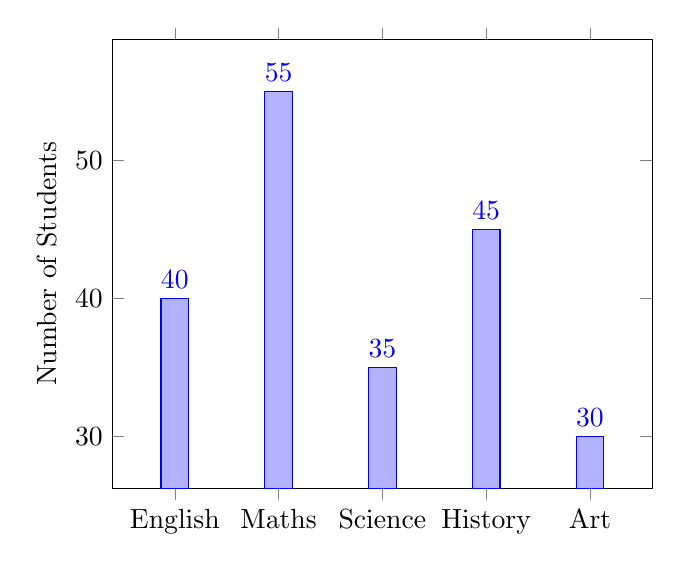
\begin{tikzpicture}
\begin{axis}[
    ybar,
    enlargelimits=0.15,
    ylabel={Number of Students},
    symbolic x coords={English,Maths,Science,History,Art},
    xtick=data,
    nodes near coords,
    nodes near coords align={vertical},
]
\addplot coordinates {(English,40) (Maths,55) (Science,35) (History,45) (Art,30)};
\end{axis}
\end{tikzpicture}

\item What subject has the most students?
\item What is the total number of students in all subjects?


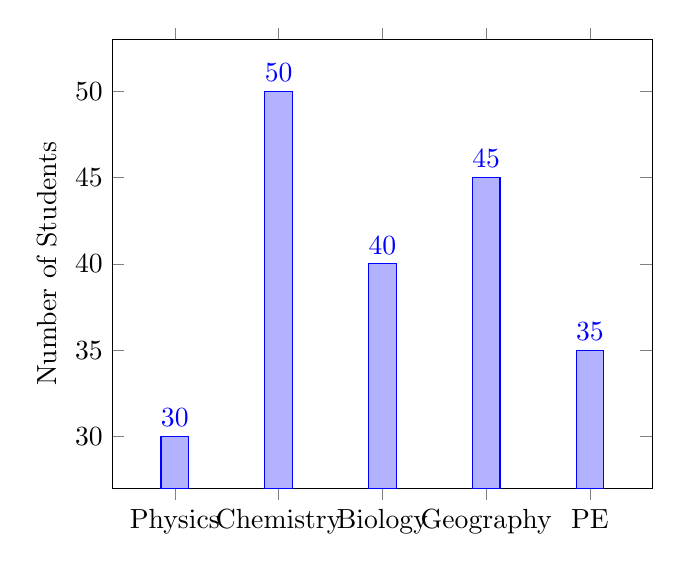
\begin{tikzpicture}
\begin{axis}[
    ybar,
    enlargelimits=0.15,
    ylabel={Number of Students},
    symbolic x coords={Physics,Chemistry,Biology,Geography,PE},
    xtick=data,
    nodes near coords,
    nodes near coords align={vertical},
]
\addplot coordinates {(Physics,30) (Chemistry,50) (Biology,40) (Geography,45) (PE,35)};
\end{axis}
\end{tikzpicture}

\item What subject has the fewest students?
\item What is the total number of students in all subjects?



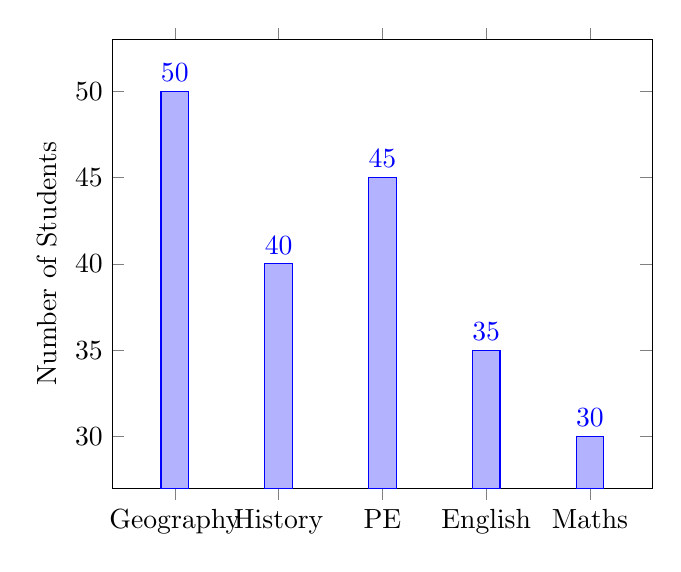
\begin{tikzpicture}
\begin{axis}[
    ybar,
    enlargelimits=0.15,
    ylabel={Number of Students},
    symbolic x coords={Geography,History,PE,English,Maths},
    xtick=data,
    nodes near coords,
    nodes near coords align={vertical},
]
\addplot coordinates {(Geography,50) (History,40) (PE,45) (English,35) (Maths,30)};
\end{axis}
\end{tikzpicture}

\item What subject has the most students?
\item What is the total number of students in all subjects?


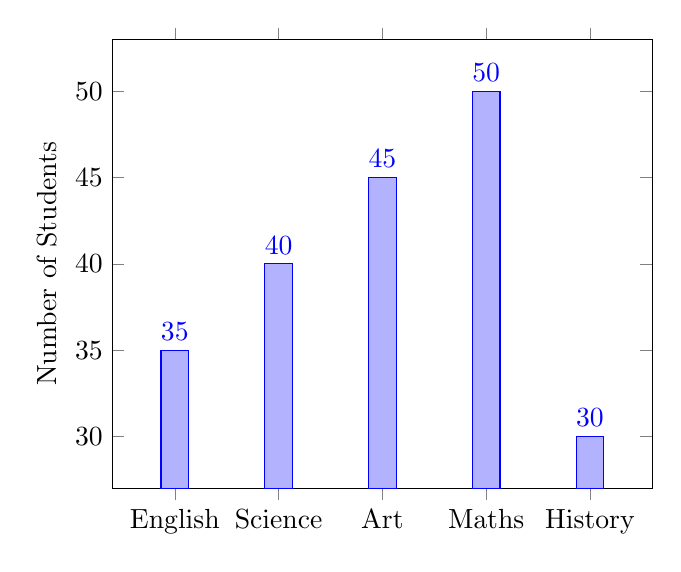
\begin{tikzpicture}
\begin{axis}[
    ybar,
    enlargelimits=0.15,
    ylabel={Number of Students},
    symbolic x coords={English,Science,Art,Maths,History},
    xtick=data,
    nodes near coords,
    nodes near coords align={vertical},
]
\addplot coordinates {(English,35) (Science,40) (Art,45) (Maths,50) (History,30)};
\end{axis}
\end{tikzpicture}

\item What subject has the fewest students?
\item What is the total number of students in all subjects?
\end{enumerate}

\end{document}
